
\Minisec{DNS}
Namensraum:bis 255 Zeichen aus verketteten Labels; \\
Labels: 1-63 Zeichen aus a-z,0-9 und -; Sonderzeichen mit Punycode\\
Records: Zuordnugstabellen Typen: A (IPv4) AAAA (IPv6) PTR (Reverse Lookup) ...

\minisec{organisatorische Struktur:} aufteilung in Zonen (Domain und darunterliegende Hosts); \\
jede Zone hat eigene Nameserver, Verantworlichen und Namenskonventionen\\
Nameserver kennen: direkt untergeordnete Hosts und Nameserver;  Root-Server


\minisec{Auflösungsmechanismus:}
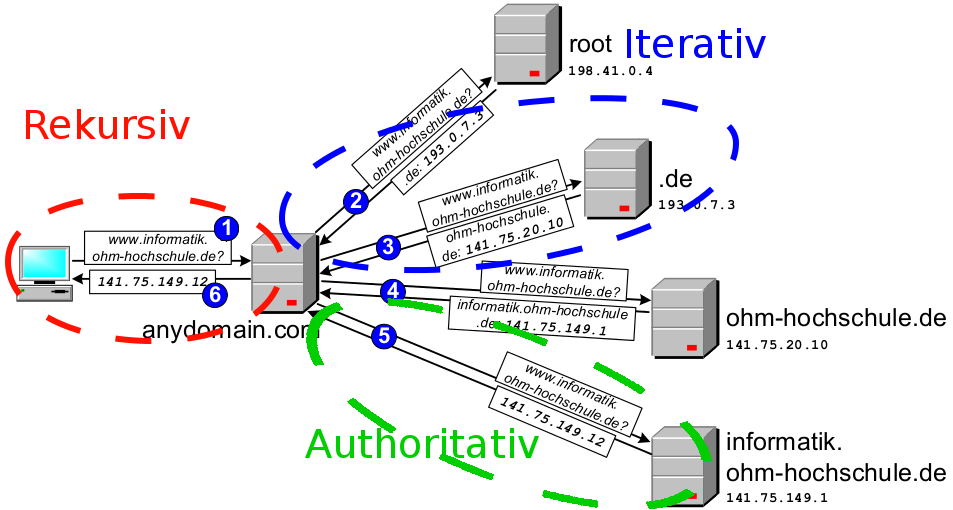
\includegraphics[width=0.3\textwidth]{DNS}

\minisec{Reverse-Lookup:}
Umwandeln der IP-Adresse in spezielle Domain, anfrage in Record PTR\\
TLDs: in-addr.arpa, ip6.arpa\\
z.B. 141.75.201.12 $\rightarrow$ 12.201.75.141.in-addr.arpa 

\Minisec{DNSsec}
Antwort wird signiert, Schlüssel durch nächsthöheren DNS bestätigt \\
2 Schlüsselpaare (Erleichtert Schlüsseltausch, kurze Schlüssel möglich):\\
\textbf{ZSK} (Zone Signing Key): Signieren der Antworten (kurz, Änderung Tage-Wochen), Tausch hat nur lokale Auswirkungen\\
\textbf{KSK} (Key Signing Key): Signieren der Schlüssel (lang, Änderung Jahre), Bei Tausch absprache mit übergeordneten Domain

\textcolor{red}{\textbf{DS}} (Delegation Signer): Mit ZSK signierter öffentlicher KSK der \textbf{Subdomain}

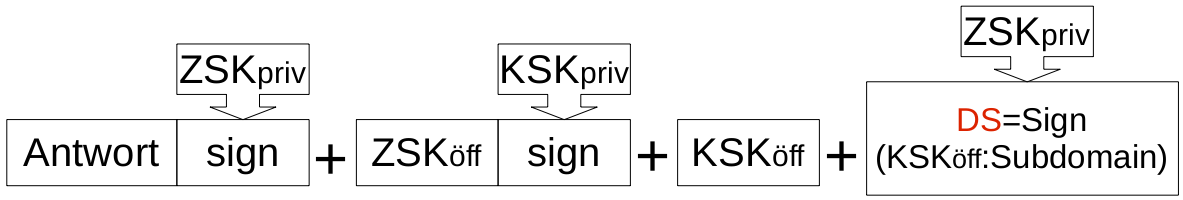
\includegraphics[width=0.4\textwidth]{DNSsec}

\Minisec{URL}
Protokoll :// Benutzer : Passwort @ Domain : Port / Pfad ? Anfrage \# Abschnitt